\section{Introduction}\label{sec:intro}

A lattice L\'evy walk moves on $\Z$ in runs of alternating direction. The run
lengths are independent, the right runs have one law and the left runs another,
and we assume that both tails are regularly varying with the same index
$\alpha\in(0,1)$. So the runs have infinite mean. Let $A_N$ be the number of right
steps among the first $N$, and put $P_N(k)=\Prob(A_N=k)$ for $0\le k\le N$. The
walk is at $2A_N-N$ after $N$ steps, so $P_N$ is the law of the walk on its natural
lattice, and it is also the law of the occupation count of a discrete-time
alternating renewal process. In the infinite-mean regime $A_N/N$ does not
concentrate. Its limit law is a generalized arcsine law, with density
\begin{equation}\label{eq:lamperti-intro}
 \La(x)=\frac{\sin\pi\alpha}{\pi}\,
 \frac{b\,x^{\alpha-1}(1-x)^{\alpha-1}}{b^2x^{2\alpha}+2b\cos(\pi\alpha)\,x^\alpha(1-x)^\alpha+(1-x)^{2\alpha}},
 \qquad 0<x<1,
\end{equation}
where $b$ is the limit ratio of the left tail to the right tail. This density goes
back to Lamperti~\cite{lamperti1958}, and in the physics literature it is called
the Lamperti distribution~\cite{margolinbarkai2006,zdk2015}. This paper is about
the local form of this law, at single points $k$.

\subsection{The local Lamperti law}\label{sec:intro-local}

Write $T_\pm(n)=\Prob(X_\pm\ge n)$ for the tails of the two run lengths. A renewal
law with a tail $T$ of index $\alpha\in(0,1)$ satisfies the strong renewal theorem
(SRT) if its renewal mass function $u$ satisfies
\[
 u(n)\sim\frac{\sin\pi\alpha}{\pi}\,\frac1{nT(n)}\qquad(n\to\infty).
\]
For $\alpha>1/2$ this always holds under aperiodicity, by Garsia and
Lamperti~\cite{garsialamperti1963} and Erickson~\cite{erickson1970}. For
$\alpha\le1/2$ it can fail, and Caravenna and Doney~\cite{caravennadoney2019}
found the exact condition. Our first theorem says that the local Lamperti law is
equivalent to the strong renewal theorem for both run laws.

\begin{introtheorem}[the local Lamperti law]\label{thm:local}
Assume that $T_\plus$ and $T_\minus$ are regularly varying with index $-\alpha$,
$0<\alpha<1$, that $T_\minus(n)/T_\plus(n)\to b\in(0,\infty)$, and that the run laws
are aperiodic. Let the walk start with a fresh run of either sign. Then the
following are equivalent.
\begin{enumerate}[(i)]
\item $NP_N(\lfloor x_0N\rfloor)\to\La(x_0)$ for one $x_0\in(0,1)$.
\item $NP_N(k)=\La(k/N)+o(1)$ uniformly over $k$ with $k/N$ in each compact
subset of $(0,1)$.
\item Both run laws satisfy the strong renewal theorem.
\end{enumerate}
\end{introtheorem}

With the theorem of Caravenna and Doney this gives a complete answer. For
$\alpha>1/2$ the local law holds under regular variation and aperiodicity alone.
For $\alpha\le1/2$ it holds if and only if each run law satisfies their condition,
which we recall in Lemma~\ref{lem:cd}, and Doney's local condition
$f_\pm(n)=O(T_\pm(n)/n)$ suffices. A single interior point already forces the
strong renewal theorem for both laws. Without it the lower half of the local law still
holds, $\liminf_N(NP_N(k)-\La(k/N))\ge0$ uniformly on compact sets, and the failure of the
strong renewal theorem shows up as an excess at every interior point
(Corollary~\ref{cor:lower}).

The proof does not need a bivariate local renewal theorem. An exact identity
writes $P_N(k)$ through the convolution powers of the two run laws, sorted by the
number $m$ of completed runs. For $m$ of order $1/T_\plus(N)$ the local limit
theorem of Gnedenko gives a Riemann sum for an explicit double integral. The key
estimate, Lemma~\ref{lem:key}, bounds the probability that the $(m+1)$-th run covers
a level $k$ by $CT(k)$ uniformly in $m$, under regular variation alone. It
decouples the two signs for small $m$, and the contribution of small $m$ of each
sign is then exactly the quantity that Caravenna and Doney show to be
asymptotically negligible if and only if the strong renewal theorem holds. The
limit comes out as a double integral over stable densities, and we identify it
with $\La$ through its Stieltjes transform (Proposition~\ref{prop:lambda}). This
gives a self-contained derivation of Lamperti's density in this setting.

\subsection{The shape}\label{sec:intro-shape}

For equal tails, $b=1$, the density $L_{\alpha,1}$ is U-shaped for small $\alpha$
and has an interior maximum at $1/2$ for $\alpha$ close to $1$. Margolin and
Barkai~\cite{margolinbarkai2006} state that the transition happens at
$\alpha=0.5946\ldots$, and the review of Zaburdaev, Denisov and
Klafter~\cite{zdk2015} says that the shape is W-like for $\alpha\gtrsim0.6$. We
give the threshold in closed form and prove the exact count.

\begin{introtheorem}[the shape]\label{thm:shape}
$L_{\alpha,1}$ has exactly $1$ critical point, a minimum at $1/2$, if
$\cos(\pi\alpha/2)\ge\alpha$, that is if $\alpha\le\alpha_c=0.5946116440\ldots$.
For $\alpha>\alpha_c$ it has exactly $3$, a strict local maximum at $1/2$ and two
strict minima placed symmetrically.
\end{introtheorem}

The proof reduces the derivative to a function of one variable that is strictly
increasing. Figure~\ref{fig:shape}(a) shows the density on both sides of the threshold.

\begin{figure}[t]
\centering
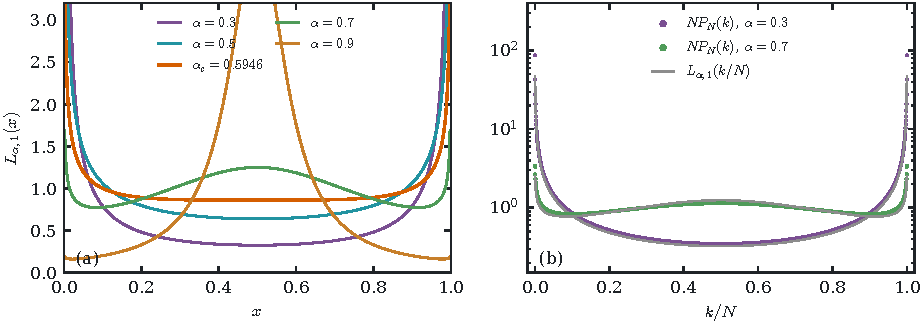
\includegraphics[width=\textwidth]{shape}
\caption{(a) The density $L_{\alpha,1}$ for $\alpha=0.3$, $0.5$, $\alpha_c$, $0.7$ and $0.9$.
At $\alpha_c$ the minimum at $1/2$ is flat to second order. (b) The exact law $NP_N(k)$ for
$N=2000$, the zeta law $f(n)\propto n^{-\alpha-1}$ for both signs and the fair start, with
$\alpha=0.3$ and $\alpha=0.7$, on a logarithmic scale, together with $L_{\alpha,1}(k/N)$. The
end values are of order $NT(N)$ and lie far above the density for $\alpha=0.3$.
Section~\ref{sec:verify} describes the computations.}
\label{fig:shape}
\end{figure} The discrete law $P_N$ has more structure near the ends. At distance
$j$ from the plus end it is the tail $T_\plus(N)$ times a renewal mass function
(Theorem~\ref{thm:ends}). Under Doney's condition this boundary layer matches the
bulk uniformly up to distance $o(N)$ from the end, and $NT_\plus(N)\to\infty$ makes
the end values much larger than the bulk values. So the global mode lies at bounded
distance from an end for every $\alpha\in(0,1)$ (Corollary~\ref{cor:mode}). For
$1<\alpha<2$ the same comparison has a golden ratio threshold~\cite{pemmasaniF}, and
here it has none. The ends also add local extrema of their own.
Theorem~\ref{thm:signs} gives a lower bound on the number of sign changes of
$k\mapsto P_N(k+1)-P_N(k)$, as the critical points of $\La$ plus the sign changes of
the two end profiles. Conjecture~\ref{conj:count} states that the bound is exact
for large $N$. It matches every case we computed.

\subsection{The initial run}\label{sec:intro-initial}

Wang, Schulz, Deng and Barkai~\cite{wsdb2018} studied renewal processes with
fat-tailed sojourn times in continuous time and left ``the effect of initial
preparation on the rare fluctuations'' for future work~\cite[Section~VIII]{wsdb2018}.
For the occupation count with $1<\alpha<2$ this is answered in~\cite{pemmasaniF}.
Theorem~\ref{thm:initial} treats $0<\alpha<1$. Let the first run have sign $\sgn$
and length $d$ with probability $\nu_\sgn(d)$. In the finite-mean case the bulk
needs no condition on the initial run on any macroscopic interior. Here it does.
A first run that ends just before the $k$-th plus step leaves a remainder that sits
in its own boundary layer, where the probabilities are of order $T(N)$ and not
$1/N$. Theorem~\ref{thm:initial} gives the exact defect in the bulk, the necessary
condition $\nu_\pm(n)=o(1/(nT_\plus(n)))$, the sufficient condition $n\nu_\pm(n)\to0$
under Doney's condition, and an exact criterion. It also shows by example that an
initial run which is finite almost surely can change the local law at interior
points, and that the necessary condition is not sufficient. At the ends the
criterion becomes the window condition
$\sum_{m<N/2}\nu_\plus(N-m)T_\plus(m)=o(T_\plus(N))$. Under Doney's condition every
fixed initial run with $n\nu_\pm(n)\to0$ leaves the local law and the end layers unchanged. An initial run
of length of order $N$ should change the local law itself, by an explicit mixture,
and we state this as Conjecture~\ref{rem:aging}.

\subsection{Related work}\label{sec:intro-related}

\emph{Occupation times.} Lamperti~\cite{lamperti1958} proved an occupation time
theorem for a class of stochastic processes, and the generalized arcsine density
$\La$ is attached to his name~\cite{margolinbarkai2006,zdk2015}. Mitov and
Yanev~\cite{mitovyanev2001} study limit theorems for the occupation-time process of
alternating renewal processes when the mean cycle is infinite, extending results of
Dynkin, Lamperti and Erickson for the spent lifetime. Starreveld, Bekker and
Mandjes~\cite{sbm2018} give the transform of the occupation time of an alternating
renewal process at an exponential time, a central limit theorem under finite second
moments, large deviations, and applications to L\'evy processes. Godr\`eche and
Luck~\cite{godrecheluck2001} give the transform of the occupation time and its limit
laws. All of these are statements in distribution. We found no local limit theorem
for the occupation count of an alternating renewal process with infinite means.

\emph{Strong renewal theorems.} The strong renewal theorem for $\alpha>1/2$ is due
to Garsia and Lamperti~\cite{garsialamperti1963}, Williamson~\cite{williamson1968}
and Erickson~\cite{erickson1970}. Doney~\cite{doney1997} proved it for all
$\alpha\in(0,1)$ under the local condition $f(n)=O(T(n)/n)$, together with a local
large deviation bound. Caravenna and Doney~\cite{caravennadoney2019} gave the
necessary and sufficient condition for $\alpha\le1/2$, and their local large
deviation bound for sums of a fixed number of variables is the main input of our
key estimate. Berger~\cite{berger2019ptrf} extends Doney's local bound, and his
version is the one we quote. Berger~\cite{berger2019} also proved multivariate
strong renewal theorems. Theorem~\ref{thm:local} shows that for the occupation count
the bivariate problem reduces exactly to the two univariate ones.

\emph{Physics.} In the physics literature the walk is the L\'evy walk in the ballistic
regime~\cite{zdk2015}, and the occupation count is the time average of a blinking
signal with power-law sojourn times~\cite{margolinbarkai2006}. Both sources use
$L_{\alpha,1}$ as the limit density of the time average. Wang, Schulz, Deng and
Barkai~\cite[Section~VII.A]{wsdb2018} found an atom with a boundary layer for the
occupation time when $0<\alpha<1$, for one sojourn law and a start of fair random
sign, through a double Laplace transform. Theorem~\ref{thm:ends} is a lattice
version of this layer at a fixed time, for two laws, with the uniform matching to
the bulk.

\emph{The finite-mean case.} For $1<\alpha<2$ the occupation law has a stable bulk,
big-jump zones and boundary layers, and its initial-run dependence and modes are
described in~\cite{pemmasaniF}. We use the exact identities of that paper and recall
them with proofs in Section~\ref{sec:identities}.

\emph{Organization.} Section~\ref{sec:setting} fixes notation and proves the exact
identities. Section~\ref{sec:tools} collects the cited theorems and proves the
elementary bounds, including the key estimate. Section~\ref{sec:local} proves
Theorem~\ref{thm:local}, Section~\ref{sec:shape} proves Theorem~\ref{thm:shape},
Section~\ref{sec:ends} treats the ends and the global mode, Section~\ref{sec:initial}
treats the initial run, and Section~\ref{sec:signs} counts sign changes.
Section~\ref{sec:verify} describes the computations. No proof uses a computed number.
